% Chapter 1

\chapter{Introducción general} % Main chapter title

\label{Chapter1} % For referencing the chapter elsewhere, use \ref{Chapter1} 
\label{IntroGeneral}
Para entender este trabajo es necesario describir ciertos conceptos, explicarlos y comparar herramientas para conocer cuáles nos ofrecen mejores prestaciones para el desarrollo de una solución tecnológica en la gestión eficiente de la energía eléctrica. 
%----------------------------------------------------------------------------------------

% Define some commands to keep the formatting separated from the content 
\newcommand{\keyword}[1]{\textbf{#1}}
\newcommand{\tabhead}[1]{\textbf{#1}}
\newcommand{\code}[1]{\texttt{#1}}
\newcommand{\file}[1]{\texttt{\bfseries#1}}
\newcommand{\option}[1]{\texttt{\itshape#1}}
\newcommand{\grados}{$^{\circ}$}

%----------------------------------------------------------------------------------------

%\section{Introducción}

%----------------------------------------------------------------------------------------

\section{Conceptos generales}

En esta sección se describen aspectos esenciales para poder conocer y entender las tecnologías y servicios usados en el trabajo.

\subsection{IoT y computación en la nube}

Internet de las Cosas (IoT) y la computación en la nube (\emph{Cloud Computing}) son dos conceptos y soluciones que cada día ocupan una mayor importancia en el desarrollo tecnológico industrial y empresarial, pero antes de abordar su rol e importancia es importante definirlas:



\begin{itemize}
\item Internet de las Cosas (IoT): hace referencia a una tecnología basada en la conexión de objetos cotidianos a Internet que intercambian, agregan y procesan información sobre su entorno físico para proporcionar servicios de valor añadido a los usuarios finales. También reconoce eventos o cambios, y tales sistemas pueden reaccionar de forma autónoma y adecuada \citep{BOOK:1}.

IoT es un conjunto de tecnologías que facilita la integración de sensores y actuadores que nos informan del estado de elementos cotidianos, como electrodomésticos, vehículos, herramientas o incluso seres vivos. Nos permite interactuar con ellos, habilitando su conectividad con plataformas en la nube que reciben y procesan la información para, tras su análisis, poder tomar decisiones.

\item Cloud Computing: la computación en la nube como paradigma proporciona a las empresas y usuarios soluciones informáticas (como \emph{software}, almacenamiento de datos, capacidad de procesamiento, etc.) a través de internet que son fácilmente escalables bajo demanda. Los documentos, correos electrónicos y otros datos, así como las aplicaciones informáticas, se almacenarán ``en la nube'', es decir, en línea, de modo que se puede acceder a los mismos desde cualquier ordenador o dispositivo móvil \citep{BOOK:1}.

La generalización del \emph{Cloud Computing} en la infraestructura TIC (tecnologías de información y comunicación) habilita la viabilidad de ejecutar aplicaciones completamente en Internet. En particular, permite flexibilidad de acceso \citep{BOOK:1}.

La computación en la nube es una tecnología que permite acceso a \emph{software}, almacenaje de ficheros y procesamiento de datos a través de Internet, siendo una opción alternativa a la ejecución en un servidor local. 

En el modelo de nube, no es necesario instalar aplicaciones de forma local en computadoras.

\end{itemize}

\subsection{Sensores y redes inalámbricas}

En la revolución de la industria conectada (Industria 4.0) cada vez existe una mayor oferta de sensores inteligentes que, además de medir la magnitud en cuestión, llevan integrado un circuito electrónico compatible con los estándares de comunicaciones más habituales en el mundo de IoT. Capturar datos y métricas siempre ha sido una necesidad en el mundo de los procesos y operaciones industriales.

\begin{itemize}
\item Sensores: son dispositivos capaces de convertir el mundo real (físico/químico) en el mundo digital (electrónico), nos permiten llevar la realidad a una dimensión que podemos gestionar para finalmente tomar decisiones e, incluso, actuar sobre el propio entorno. Son equipos que convierten la magnitud de entrada (temperatura, humedad, nivel, presión, etc.) en una señal eléctrica medible e interpretable por los dispositivos electrónicos.

\item Redes inalámbricas: las redes inalámbricas (\emph{Wireless}) logran propagar la conexión entre dispositivos a través de medios no físicos, usan diferentes tecnologías como las ondas electromagnéticas, radiación y medios ópticos para su transferencia. Existen varios tipos de redes inalámbricas con diferentes alcances y funcionalidades.

\end{itemize}

\subsection{Tipos de redes de IoT}

Podemos clasificarlas en dos categorías:
\begin{enumerate}
\item Redes de corto alcance y bajo consumo 

Las redes de baja potencia y corto alcance están indicadas para hogares, oficinas y otros entornos de reducido tamaño. Normalmente, necesitan baterías pequeñas y su usó suele resultar económico \citep{WEBSITE:15}. Por ejemplo:

\begin{itemize}
\item Bluetooth
\item Z-Wave
\item NFC
\item ZigBee
\item Wi-Fi/802.11
\end{itemize}

%\vspace{1cm}

\item Redes de área extensa de bajo consumo (LPWAN)

Las redes LPWAN permiten la comunicación en un radio mínimo de 500 metros, tienen un consumo de energía mínimo y se usan para la mayoría de los dispositivos IoT \citep{WEBSITE:15}. 

Los siguientes son algunos ejemplos comunes de redes LPWAN:

\begin{itemize}
\item 4G LTE para IoT
\item 5G para IoT
\item Cat-0
\item Cat-1
\item LoRaWAN
\item LTE Cat-M1
\item Sigfox
\item Banda estrecha o NB-IoT/Cat-M2
\end{itemize}

\end{enumerate}

\vspace{0.5cm}

La distancia a la que los datos deben viajar (corta o larga) determina el tipo de conectividad necesaria para un proyecto de IoT.


\section{Motivación}
Al encender cualquier dispositivo eléctrico u electrónico se produce un consumo de energía eléctrica que normalmente se desconoce. Simplemente a final de mes, se recibe la factura de consumo eléctrico, donde se indica el consumo mensual y el monto a pagar. A muchas de las empresas que tienen procesos industriales les ocurre lo mismo y es que el control del consumo de manera precisa no está normalizado en el ámbito doméstico (\emph{smart home}) y sigue siendo un aspecto aun por mejorar. Este control es muy importante ya que gracias a él podemos mejorar la eficiencia energética, ahorrando dinero para una familia o una empresa y a la vez siendo respetuosos con el medio ambiente.

Bajo ese contexto antes y durante la pandemia por el Covid-19, se registraron miles de quejas por montos excesivos en los recibos de energía eléctrica en muchos departamentos en el país de Perú. Antes de la pandemia, una usuaria de LUZ DEL SUR pagaba 80 soles al mes (\$20 USD al cambio actual) por el servicio de energía eléctrica en su vivienda en la ciudad de Lima. Ahora, pretenden cobrarle 180 soles por mes (\$45 USD al cambio actual). Cuando el usuario quiso reclamar, la empresa responsable de brindar el servicio no le contestaba. Algo parecido le pasó a una asociación de comerciantes a la que, a pesar de que su establecimiento estaba cerrado desde el 16 de marzo del 2020, la empresa EDELNOR pretende cobrarle 250 soles (\$ 62 USD al cambio actual) por consumos no realizados durante el mes. Estos son algunos de los miles de denuncias de consumidores que se han hecho públicas en el país de Perú  \citep{WEBSITE:1}.

Entre el 16 de marzo y fines de junio de 2020, cuando el Gobierno peruano declaró el Estado de Emergencia Nacional por el COVID-19, las empresas generadoras de electricidad dejaron de enviar a su personal a las viviendas para realizar la lectura de los consumos en los medidores de energía eléctrica de los predios y facturaron por el consumo promedio de los seis meses anteriores. En muchos casos se encontró que los consumos normales habían crecido enormemente, en otros se duplicaron y hasta se triplicaron. Este aparente sinceramiento de los consumos generó miles de reclamos por cobros excesivos como se ilustra con la figura \ref{fig:noticia}. 

El mayor número de reclamos de los usuarios se presentó en julio y agosto de 2020. En solo una semana, el Organismo Supervisor de la Inversión en Energía y Minería (OSINERGMIN) recibió en Lima alrededor de 20 mil reclamos, tanto contra ENEL como por LUZ DEL SUR. Esta situación se repitió a nivel nacional, sobre todo en las regiones de Puno, La Libertad, Áncash y Ucayali \citep{WEBSITE:1}.

%\vspace{1cm}
\begin{figure}[htbp]
\centering
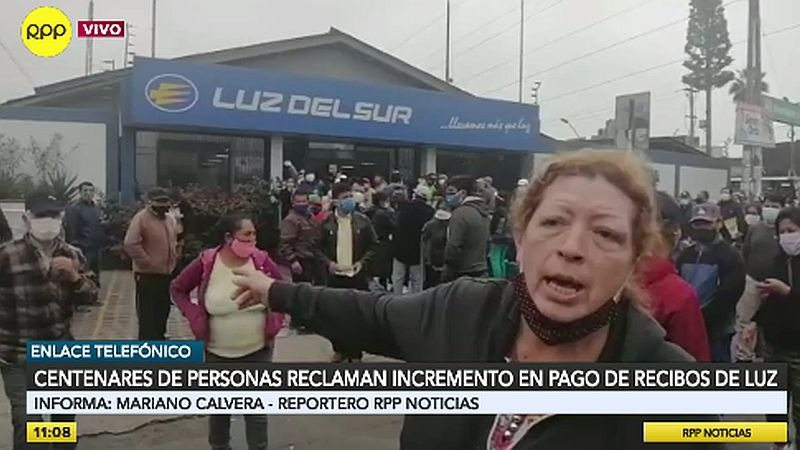
\includegraphics[width=.7\textwidth]{./Figures/motivacion.jpg}
\caption{Noticias de la problemática en Lima Perú \protect\footnotemark.}
\label{fig:noticia}
\end{figure}
%\vspace{1cm}
\footnotetext{Imagen tomada de \url{https://rpp.pe/noticias/luz-del-sur}}

El organismo supervisor del estado recordó que en los casos donde la lectura del medidor confirme que el consumo real ha sido menor al facturado, la empresa deberá devolver lo pagado en exceso en una sola oportunidad o proceder a refacturar \citep{WEBSITE:2}.

Realizar el proceso de refacturación para corregir estos errores costará demasiado tiempo y dinero al estado y a las empresas que ofrecen dicho servicio, presentando incomodidad y daño económico a toda la población afectada. 

Como parte de los usuarios afectados en esta problemática en Perú, surge la necesidad de desarrollar un sistema de monitoreo y control que permita conocer el consumo eléctrico mensual detallado, siendo este una herramienta automatizada de respaldo y que sirva como evidencia para prevenir facturaciones erróneas para hogares, edificios habitacionales, empresas, etc.

%-----------------------------------------------------------------------
\section{Estado del arte}

A continuación, se describen soluciones que son utilizadas en el control del consumo eléctrico y que están actualmente en el mercado comercial. 

Para una mejor comprensión se los clasifica en dos categorías:

\begin{itemize}
\item Sistemas de monitoreo para gestión de energía eléctrica.
\item Módulos independientes para gestión de energía eléctrica.
\end{itemize} 

\subsection{Sistemas de monitoreo para gestión de energía eléctrica}
Los sistemas de monitoreo son sistemas integradores automatizados compuestos por un \emph{software} de control y monitoreo, sensores y actuadores, por ejemplo:

\begin{itemize}
\item \keyword{Energy Vision}: solución de \emph{software} para gestión del consumo de energía. Energy vision - Centraline es una nueva herramienta de \emph{software} de gestión energética profesional con el fin de lograr un ahorro importante y maximizar la eficiencia energética. El sistemas se ilustra con la figura \ref{fig:energy-vision} 
%\vspace{0.5cm}
\begin{figure}[htbp]
\centering
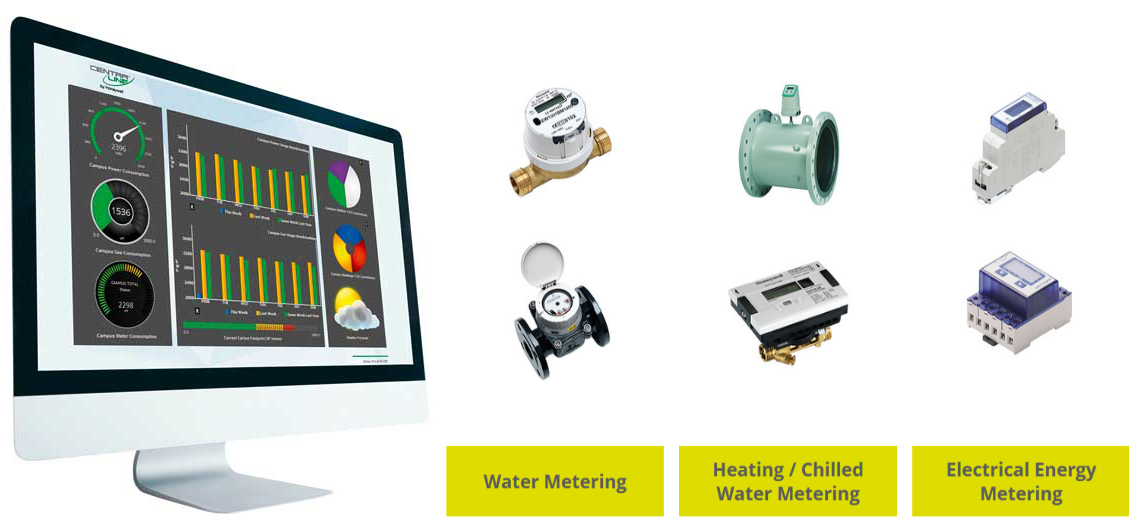
\includegraphics[width=.9\textwidth]{./Figures/energy-vision.jpg}
\caption{Sistema y productos Energy Vision \protect\footnotemark}
\label{fig:energy-vision}
\end{figure}

\footnotetext{Imagen tomada de \url{https://www.centraline.com/itIT/prodotti-e-documentazione/special/energy-vision-nx.html}}


El \emph{software} permite recopilar y analizar todas las formas de uso de energía para una gestión energética profesional y constituye un componente esencial en la automatización de edificios eficientes desde el punto de vista energético \citep{WEBSITE:13}. Esta herramienta de \emph{software} contiene gráficos y diagramas visualmente atractivos y proporcionan una presentación ordenada y fácil de comprender de la información que se necesita. Recopila, archiva, evalúa y consulta todos los datos de un edificio. 

Se puede acceder al sistema desde todo tipo de dispositivos mediante un navegador con Internet.

%\vspace{1cm}
%\vspace{1cm}

\item \keyword{Iammeter}: sistema de monitoreo de energía.

Iammeter es un sistema de monitoreo de energía dedicado, al que se puede conectar medidores de energía Wi-Fi y luego comenzar a rastrear el uso de electricidad de su hogar o edificio comercial, y monitorear el flujo de energía del sistema fotovoltaico solar \citep{WEBSITE:11}.

El sistema Iammeter puede generar un análisis integral del consumo de energía por usuarios, ofreciendo gráficos de datos y algunos detalles en el panel de información general. Ofrece el cálculo de la factura de la luz diaria/mensual y monitoreo en tiempo real del uso de electricidad \citep{WEBSITE:12}. El sistema se ilustra con la figura \ref{fig:iammeter}.

\vspace{0.5cm}

\begin{figure}[htbp]
	\centering
	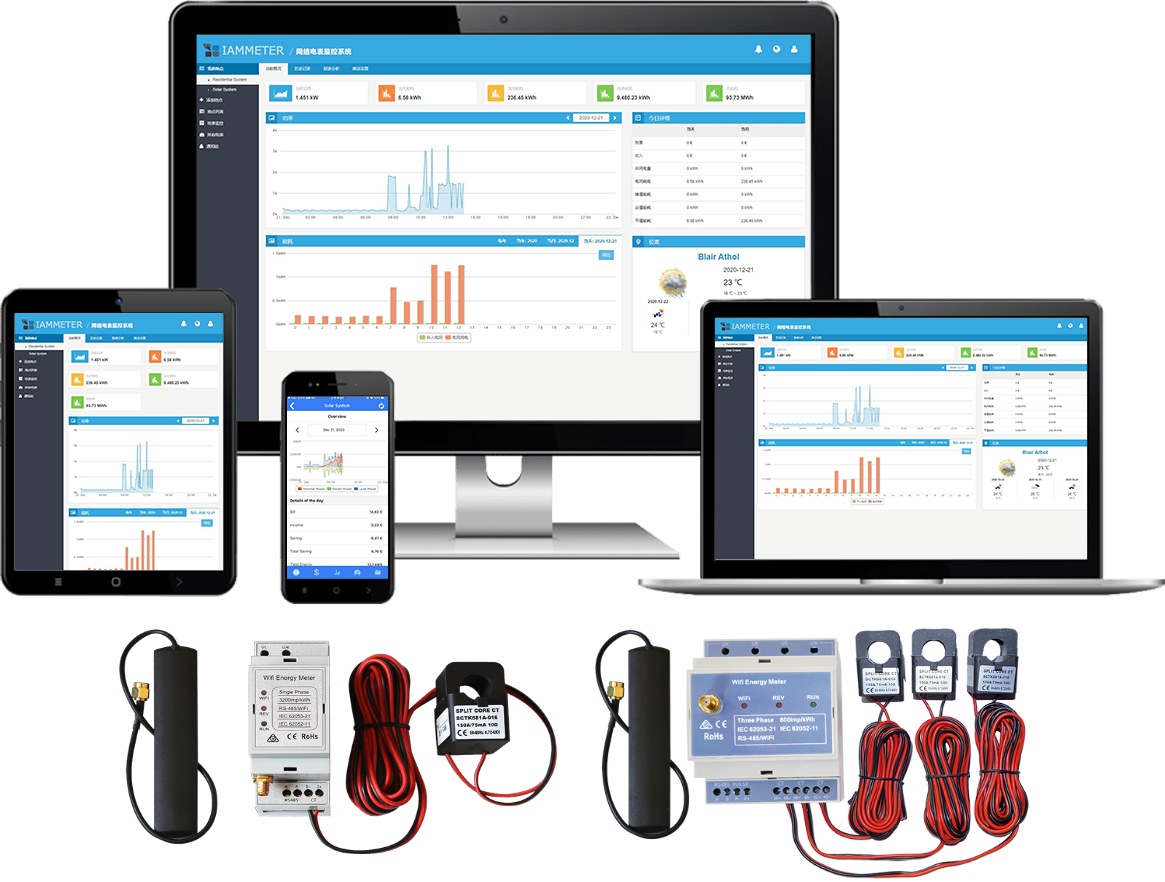
\includegraphics[width=.9\textwidth]{./Figures/iammeter.png}
	\caption{Sistema y productos Iammeter \protect\footnotemark.}
	\label{fig:iammeter}
\end{figure}
\vspace{0.5cm}

\footnotetext{Imagen tomada de \url{https://es.iammeter.com/}}

Se puede acceder sistema desde todo tipo de dispositivos mediante un navegador con Internet o mediante su aplicación móvil.
\vspace{1cm}
\vspace{1cm}

\item \keyword{Bee2energy}: gestión de eficiencia energética.

El sistema Bee2energy de la empresa Compta ofrece un servicio integral de \emph{software} que permite a las empresas e instituciones lograr mejoras significativas en el uso de la eficiencia energética a la vez que minimiza los impactos ambientales, reduciendo los consumos y los costos operativos \citep{WEBSITE:14}. El sistema se ilustra con la figura \ref{fig:bee2energy}. 

\begin{figure}[htbp]
	\centering
	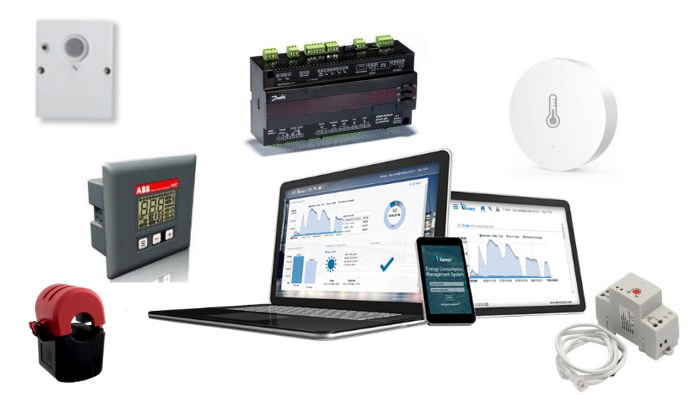
\includegraphics[width=.8\textwidth]{./Figures/bee2energy.jpg}
	\caption{Sistema y productos Bee2energy \protect\footnotemark.}
	\label{fig:bee2energy}
\end{figure}

\footnotetext{Imagen tomada de \url{https://www.ceb-solutions.com/es/productos/bee2energy/}}

Bee2energy es una solución IoT basada en la nube a la que se puede acceder en cualquier momento y en cualquier lugar a través de Internet. Brinda operaciones en tiempo real con un modelo de negocio SaaS (\emph{\emph{software} as a service}) flexible y con capacidad multicanal \citep{WEBSITE:14}. Las funciones de control en edificios se ilustra con la figura \ref{fig:bee2energy2}.

\begin{figure}[htbp]
	\centering
	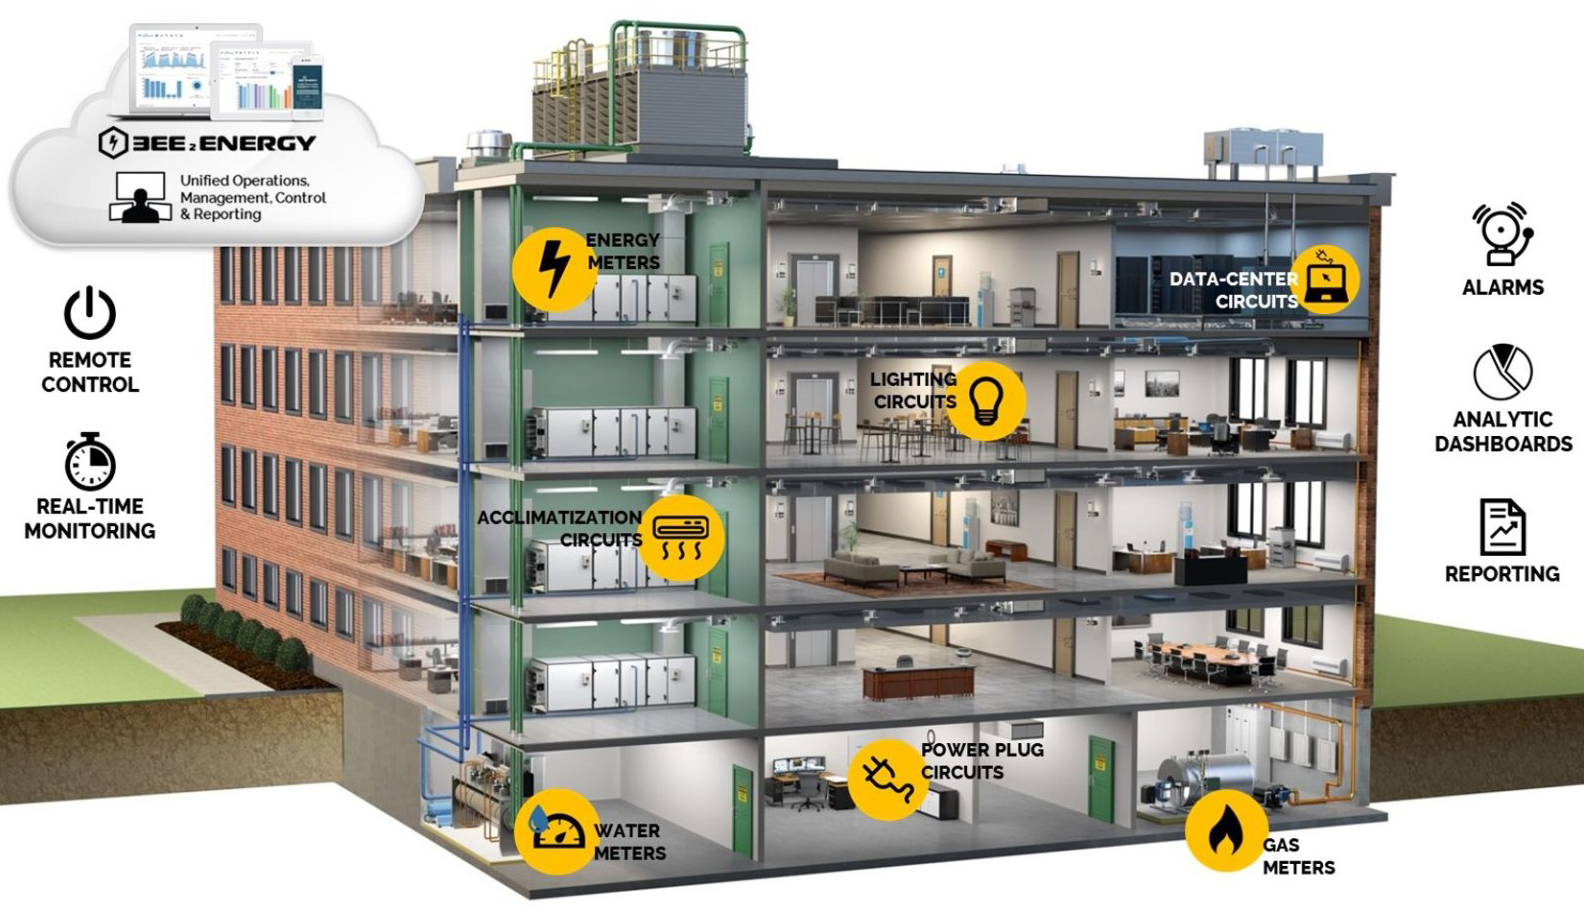
\includegraphics[width=.85\textwidth]{./Figures/bee2energy2.jpg}
	\caption{Monitoreo y control en tiempo real en edificios \protect\footnotemark.}
	\label{fig:bee2energy2}
\end{figure}

\footnotetext{Imagen tomada de \url{https://www.ceb-solutions.com/es/productos/bee2energy/}}

Ofrece monitoreo en tiempo real de consumos, temperaturas, humedad y otros indicadores, configuración de reglas y encender / apagar equipos automáticamente o configurar alarmas y notificaciones.
\end{itemize}
%----------------------------------------------------------------------------------------
\subsection{Módulos independientes para gestión de energía eléctrica}
Los módulos independientes son sensores o actuadores  que se comercializan de forma individual, puede ser un sensor de consumo, interruptores o tomacorrientes inteligentes, por ejemplo: 
\begin{itemize}

\item \keyword{Tomacorriente smart}: es la manera más sencilla de convertir en inteligentes tus dispositivos electrónicos para poder controlarlos. Simplemente se debe conectar en un tomacorriente de CA (corriente alterna) e integrarlo a la red Wi-Fi existente, no requiere un concentrador y a través de una aplicación, puedes encender y apagar las luces o electrodomésticos en forma remota desde cualquier lugar. Por ejemplo el dispositivo de la figura \ref{fig:tomacorriente}.

\begin{figure}[htbp]
	\centering
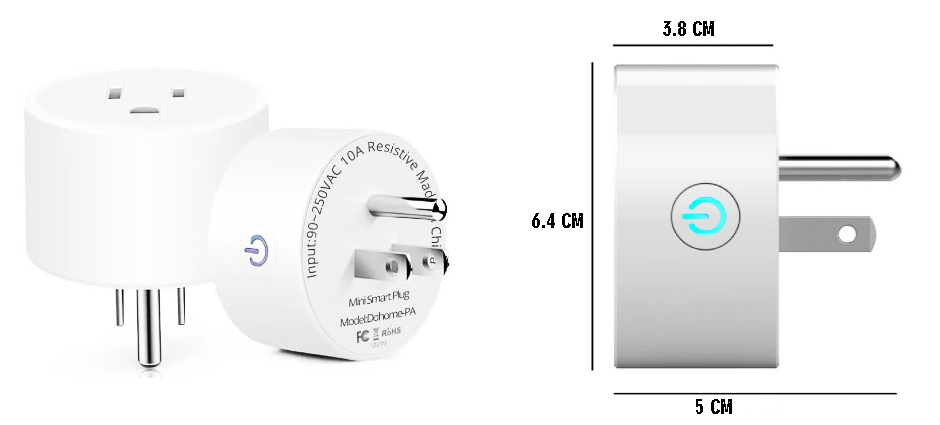
\includegraphics[width=0.8\textwidth]{./Figures/tomacorriente.png}
	\caption{Tomacorriente inteligente de facil uso \protect\footnotemark.}
	\label{fig:tomacorriente}
\end{figure}

\footnotetext{Imagen tomada de \url{https://www.promart.pe/electricidad/interruptores-y-tomacorrientes/}}

%\vspace{1cm}
%\vspace{1cm}
%\vspace{1cm}
%\vspace{1cm}
%\vspace{1cm}
%\vspace{1cm}
%\vspace{1cm}
%\vspace{1cm}



\item \keyword{Medidor digital eléctrico monofásico}: es un medidor tipo electrónico con cubierta de policarbonato diseñado para controlar el consumo de energía de manera independiente, tiene una alta resistencia a la humedad, corrosión y temperatura. Por ejemplo el dispositivo de la figura \ref{fig:medidor}.

\begin{figure}[htbp]
	\centering
	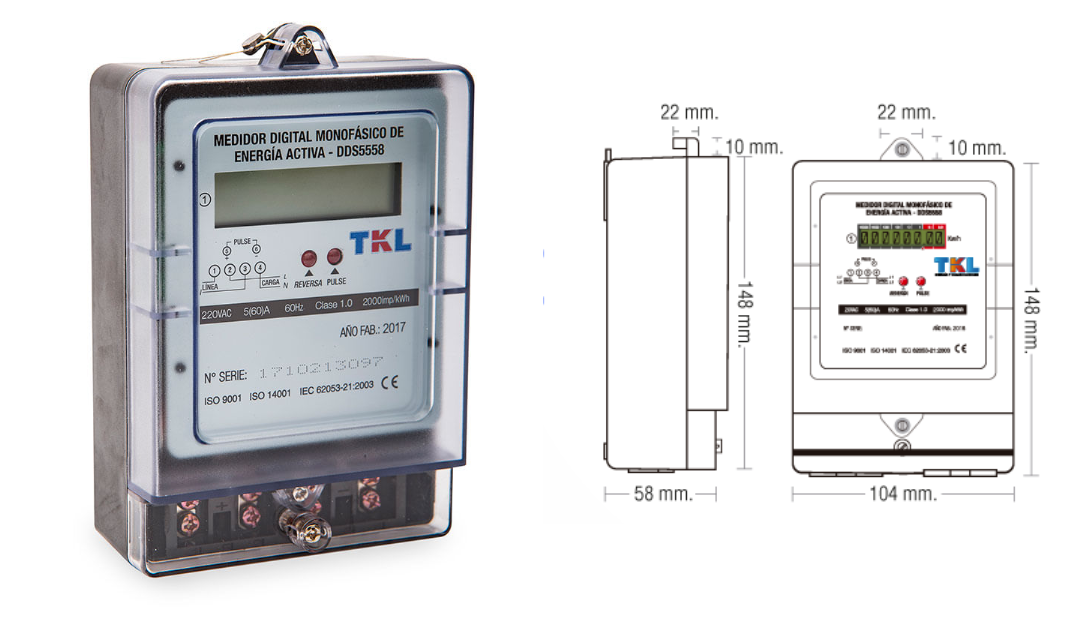
\includegraphics[width=0.9\textwidth]{./Figures/medidor.png}
	\caption{Medidor digital monofásico \protect\footnotemark.}
	\label{fig:medidor}
\end{figure}

\footnotetext{Imagen tomada de \url{https://www.promart.pe/medidor-digital-ciclometrico-60-amperios/}}

Es un medidor que incluye una pantalla LCD donde muestra la lectura de watts utilizados dentro de una vivienda, negocio u oficina.

\end{itemize}

\subsection{Comparación entre soluciones}

La comparación entre las distintas soluciones mencionadas se muestran en las tablas \ref{tab:tabla1}, \ref{tab:tabla2},  \ref{tab:tabla3} y \ref{tab:tabla4}, considerando aspectos más relevantes para conocer sus principales diferencias según su categoría. 
\begin{itemize}
\item Sistemas de monitoreo para gestión de energía eléctrica:

%%%%%%%%%%%%%%%%%%%%%%%%%%%%%%%%%%
\begin{table}[h]
	\centering
	\caption[Comparativa de soluciones entre producto y sector]{Comparativa producto y sector}
	\begin{tabular}{l c c }    
		\toprule
		\textbf{Empresa} 	& \textbf{Producto} & \textbf{Sector}  \\
		\midrule
		Honeywell International Inc & Energy Vision & Energético \\		
		Beijing Lewei IOT Technologies Co. Ltd.	 & Iammeter	& Energético solar \\
		Compta Energing Business	 & Bee2energy	& Energético \\
		\bottomrule
		\hline
	\end{tabular}
	\label{tab:tabla1}
\end{table}


%%%%%%%%%%%%%%%%%%%%%%%%%%%%%%%%%%%%%%
%escribir texto 2

\begin{table}[h]
	\centering
	\caption[Comparativa de soluciones entre acceso y servidor]{Comparativa acceso y tipo de servidor}
	\begin{tabular}{l c c c c }    
		\toprule
		\textbf{Producto} & \textbf{Acceso}  & \textbf{uso} & \textbf{S. local}   & \textbf{S. remoto} \\
		\midrule
		Energy Vision & Local y remoto 	& Navegador & No & Si  \\		
		Iammeter	 & Local y remoto	& Navegador y App. & No & Si  \\
		Bee2energy	 & Local y remoto	& Navegador & No & Si  \\
		\bottomrule
		\hline
	\end{tabular}
	\label{tab:tabla2}
\end{table}

%\vspace{1cm}
%\vspace{1cm}

%%%%%%%%%%%%%%%%%%%%%%%%%%%%%%%%%%%

%escribir texto 3

\begin{table}[h]
	\centering
	\caption[Comparativa de soluciones entre protocolo y hardware]{Comparativa protocolo y tipos de hardware}
	\begin{tabular}{l p{5cm} p{5cm}}    
		\toprule
		\textbf{Producto} 	 & \textbf{Protocolo}  & \textbf{Sensores y actuadores}  \\
		\midrule
		Energy Vision & Modbus, M-Bus  y TCP/IP 	& Propios \\		
		Iammeter	 & MQTT y TCP/IP	& Propios y compatibles con       dispositivos Sonoff   \\
		Bee2energy	 & Múltiples protocolos IoT		& Propios y compatibles con otros comerciales  \\
		\bottomrule
		\hline
	\end{tabular}
	\label{tab:tabla3}
\end{table}

\vspace{1cm}
\item Módulos independientes para gestión de energía eléctrica:


\begin{table}[h]
	\centering
	\caption[Comparativa de módulos entre protocolo y hardware]{Comparativa protocolo y tipos de hardware}
	\begin{tabular}{l p{2cm} p{3cm} p{2cm}}    
		\toprule
		\textbf{Producto} 	 & \textbf{Protocolo}  & \textbf{Función} & \textbf{Acceso} \\
		\midrule
		Tomacorriente smart & TCP/IP (Wi-Fi)	& Interruptor inteligente. & App. móvil  \\		
		Medidor digital eléctrico	 & -	& Registro de consumo.  & Presencial visual \\
		
		\bottomrule
		\hline
	\end{tabular}
	\label{tab:tabla4}
\end{table}

\end{itemize}

%----------------------------------------------------------------------------------------
\section{Identificación y análisis}



\subsection{Propósito}

El propósito de este proyecto es diseñar y desarrollar un sistema informático capaz de controlar y monitorear viviendas u otros ambientes mediante el protocolo MQTT para brindar una gestión inteligente respecto a confort y consumo energético.

\subsection{Alcance}

El proyecto incluye los siguientes ítems:
\begin{itemize}
\item Diseño y desarrollo de un módulo principal local.
\item Diseño y desarrollo del módulo replicador de datos local-nube.
\item Diseño y desarrollo del módulo actuador y de consumo.
\item Diseño y desarrollo del módulo de control de temperatura.
\end{itemize}

\subsection{Objetivos}
\begin{itemize}
\item Diseñar y desarrollar un sistema IoT para medir el consumo eléctrico.
\item Diseñar y desarrollar un sistema que no dependa de una conexión a Internet para su funcionamiento.
\item Diseñar y desarrollar un \emph{software} a medida para la gestión de control y monitoreo de una vivienda o edificio.
\item Diseñar e implementar módulos con comunicación Wi-Fi para el control y monitoreo de energía eléctrica.
\end{itemize}

%----------------------------------------------------------------------------------------
\let\cleardoublepage\clearpage % para eliminar pagina en blanco siguiente